\documentclass[10pt]{beamer}

\usepackage{polyglossia}
\usepackage{csquotes}
\usepackage{fontspec}
\usepackage{microtype}
\usepackage{color}
\usepackage{url}
\usepackage{hyperref}
\usepackage{amsfonts}
\usepackage{amsmath}
\usepackage{amsthm}
\usepackage{subcaption}
\usepackage[backend=biber,style=iso-authoryear,sortlocale=en_US,autolang=other,bibencoding=UTF8]{biblatex}
\usepackage{booktabs}

\addbibresource{zotero.bib}

\setdefaultlanguage{czech}
\setmainfont{TeX Gyre Termes}
\usetheme{Boadilla}
\usecolortheme{crane}
\setbeamertemplate{section in toc}[ball unnumbered]
\setbeamertemplate{bibliography item}{}

\hypersetup{
	pdfencoding=auto,
	unicode=true,
	citecolor=green,
	filecolor=blue,
	linkcolor=red,
	urlcolor=blue
}

\makeatletter
\newcommand*{\currentSection}{\@currentlabelname}
\makeatother

\newcommand{\mathmat}{\ensuremath{\mathbf}}

\title[Optimalizace vzdálenosti pro MIL shlukování]
{
	Optimalizace vzdálenosti pro multi-instanční shlukovací problémy
}

\titlegraphic
{
	
\includegraphics[width=0.12\columnwidth]{images/fjfi.png}
}

\date{5. února 2020}

\author[Marek Dědič]
{
	Marek~Dědič\inst{1}\inst{2} \\
	Školitel:~Doc.~Ing.~Tomáš~Pevný,~Ph.D.\inst{3}\inst{4}
}

\institute[FJFI ČVUT v Praze]
{
	\inst{1} ČVUT v Praze, Fakulta jaderná a fyzikálně inženýrská, Matematická informatika \and
	\inst{2} Cisco Systems Inc., Karlovo náměstí 10, Praha 2 \and
	\inst{3} ČVUT v Praze, Fakulta elektrotechnická \and
	\inst{4} Avast Software s.r.o., Pikrtova 1737/1a, Praha 4
}

\AtBeginSection[]{
	\begin{frame}{\currentSection}
		\tableofcontents[currentsection]
	\end{frame}
}

\begin{document}

\begin{frame}
	\titlepage
\end{frame}

% Body

\section{Motivace \& Úloha}

\begin{frame}{Motivace}
	\begin{itemize}
		\item Shluková analýza je jedním z nejzákladnějších problémů učení bez učitele.
		\item Klíčovou složkou návrhu shlukovacího algoritmu je volba vzdálenostní metriky a pro složitější úlohy je často obtížné najít správnou metriku.
		\item Multi-instanční učení je způsobem, jak efektivně konstruovat komplexní hierarchické modely cílené na specifickou úlohu.
		\item V diplomové práci byly představeny a srovnány 3 přístupy multi-instanční shlukové analýzy.
	\end{itemize}
\end{frame}

\begin{frame}{Úloha}
	\begin{itemize}
		\item Síťová bezpečnost je atraktivní aplikací navržených metod.
		\item Cílem práce bylo umožnit shlukování domén 2. řádu podle aktivity klientů, kteří se na ně připojují.
		\item Úspěšné shlukování může výrazně podpořit práci síťových analytiků.
		\item Možné budoucí rozšíření na šifrovaná data se stoupajícím šifrováním základních protokolů.
	\end{itemize}
\end{frame}

\begin{frame}{Obsah}
	\tableofcontents
\end{frame}

\section{MIL}

\begin{frame}[c]\frametitle{End--to--end učení}
	\centering
	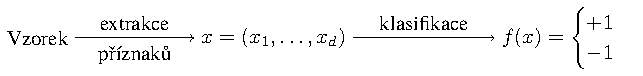
\includegraphics{images/end_to_end_learning/end_to_end_learning.pdf}
\end{frame}

\begin{frame}[c]\frametitle{Multi instanční učení}
	\centering
	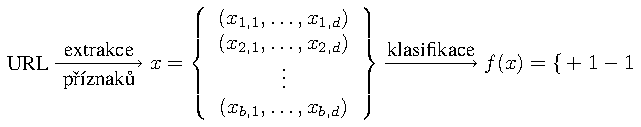
\includegraphics{images/multi_instance_learning/multi_instance_learning.pdf}
\end{frame}

\begin{frame}[c]\frametitle{Paradigma vloženého prostoru}
	\centering
	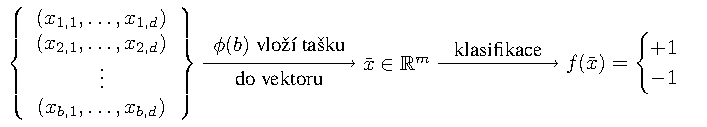
\includegraphics{images/embedded_space_paradigm/embedded_space_paradigm.pdf}
\end{frame}

\begin{frame}{Vkládající funkce \( \phi \)}
	\centering
	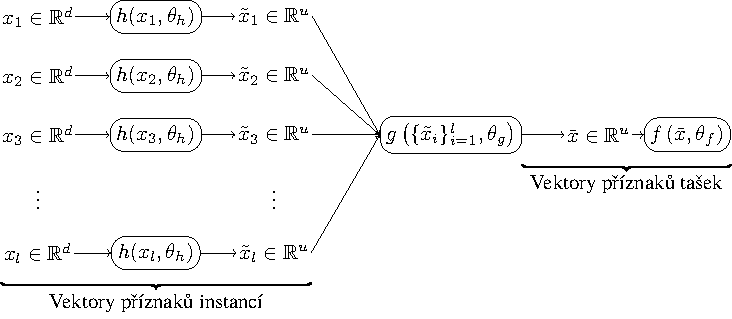
\includegraphics[width=0.9\pagewidth]{images/embedding_function/embedding_function.pdf}
\end{frame}

\section{Contrastive predictive coding}

\begin{frame}{Contrastive predictive coding}
	Vyjádření přístupu pomocí constractive predictive coding jako ztrátové funkce
	\[ \mathmat{D}_{ij} = \left\lVert \phi \left( B_i^{(1)} \right) - \phi \left( B_j^{(2)} \right) \right\rVert_2^2 \]
	\[ L_\mathrm{CPC} = \frac{1}{n} \sum_{i = 1}^n \left( \log \left( \mathmat{D}_{ii} \right) - \log \sum_{\substack{j = 1 \\ j \neq i}}^n \mathmat{D}_{ij} \right) \]
\end{frame}

\section{Triplet loss}

\begin{frame}{Triplet loss}
	Triplet loss je alternativou vyžadující supervised přístup
	\[ \mathmat{y}_{ij} =
\begin{cases}
	1 &\text{pro} \quad y_i = y_j \\
	0 &\text{jinak}
\end{cases}
\]
\[ \mathmat{\eta}_{ij} = \begin{cases}
		1 &\text{pokud taška } B_j \text{ je cílovým sousedem tašky } B_i \\
		0 &\text{jinak}
  \end{cases} \]
\[ L_\mathrm{triplet} = \sum_{ij} \eta_{ij} \mathmat{D}_{ij} + c \sum_{ijl} \eta_{ij} \left( 1 - \mathmat{y}_{il} \right) \left\{ \mathmat{D}_{il} - \mathmat{D}_{ij} \right\}_+ \]
\end{frame}

\section{Magnet loss}

\begin{frame}
	\begin{figure}[h]
		\centering
		\begin{subfigure}[b]{0.18\textwidth}
			\centering
			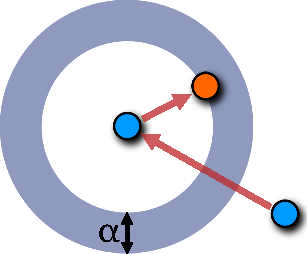
\includegraphics[width=\textwidth]{images/triplet-magnet-difference/triplet_before.pdf}
			\caption{Triplet loss: před}
		\end{subfigure}
		\hfill
		\begin{subfigure}[b]{0.18\textwidth}
			\centering
			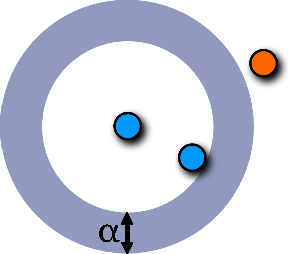
\includegraphics[width=\textwidth]{images/triplet-magnet-difference/triplet_after.pdf}
			\caption{Triplet loss: po}
		\end{subfigure}
		\hfill
		\begin{subfigure}[b]{0.18\textwidth}
			\centering
			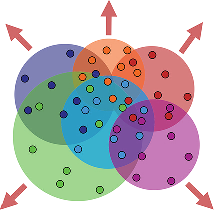
\includegraphics[width=\textwidth]{images/triplet-magnet-difference/magnet_before.pdf}
			\caption{Magnet loss: před}
		\end{subfigure}
		\hfill
		\begin{subfigure}[b]{0.18\textwidth}
			\centering
			
\includegraphics[width=\textwidth]{images/triplet-magnet-difference/magnet_after.pdf}
			\caption{Magnet loss: po}
		\end{subfigure}
		\caption{Vizualizace rozdílu mezi triplet loss a magnet loss. Obrázek z \cite{rippel_metric_2015}}
	\end{figure}
\end{frame}

\section{Výsledky}

\begin{frame}{Standardní datasety}
	\begin{figure}[h]
		\centering
		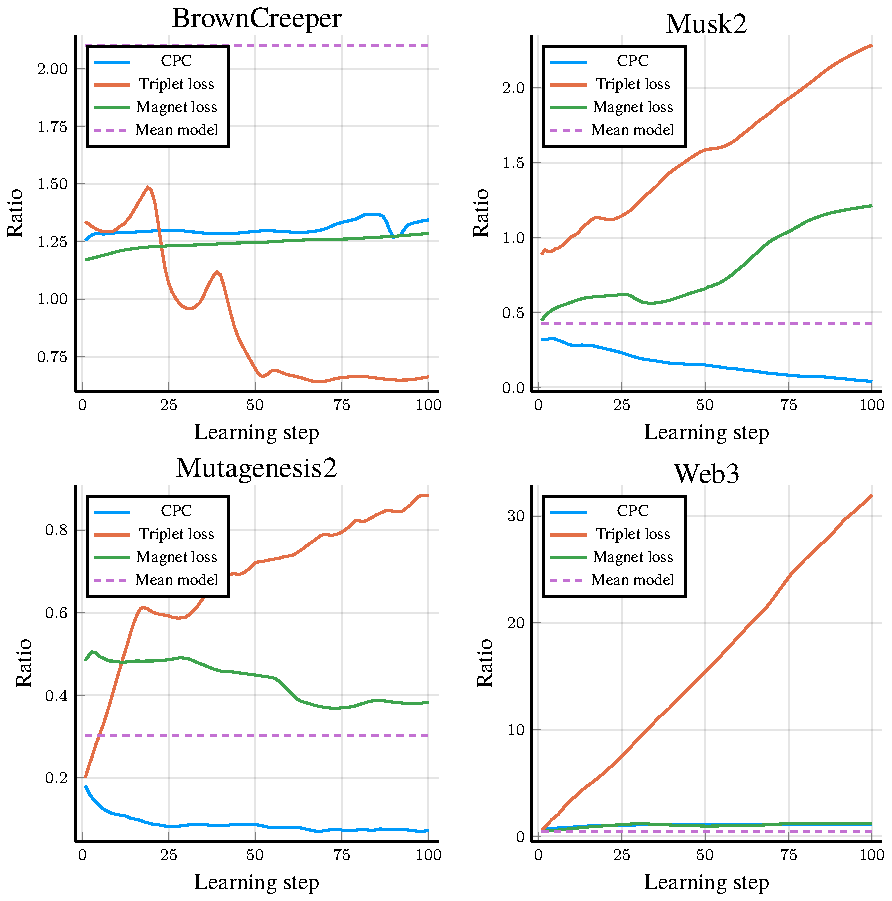
\includegraphics[width=0.55\textwidth]{images/toy-ratio/toy-ratio.pdf}
		\caption{Poměr průměrné vzdálenosti mezi shluky a průměrné vzdálenosti ve shlucích}
	\end{figure}
\end{frame}

\begin{frame}{Standardní datasety}
  \begin{table}[h]
    \begin{tabular}{lrrr}
      \toprule
      Dataset          & CPC            & Triplet loss   & Magnet loss \\
      \midrule
      BrownCreeper     & \textbf{0.900} & 0.836          & 0.818 \\
      Musk2            & 0.750          & \textbf{1.0}   & 0.650 \\
      Mutagenesis2     & 0.708          & \textbf{0.750} & 0.500 \\
      Web3             & 0.733          & \textbf{0.867} & 0.533 \\
      \bottomrule
    \end{tabular}
    \caption{Přesnost klasifikace}
  \end{table}
\end{frame}

\begin{frame}{Korporátní dataset}
  \begin{table}
    \centering
    \begin{tabular}{lrrr}
      \toprule
      Klasifikační problém & CPC   & Triplet loss & Magnet loss \\
      \midrule
      2 třídy              & 0.920 & 0.910        & \textbf{0.930} \\
      20 tříd              & 0.893 & 0.868        & \textbf{0.904} \\
      \bottomrule
    \end{tabular}
    \caption{Přesnost klasifikace}\label{tab:cisco-accuracy}
  \end{table}
\end{frame}

\section{Závěr}

\begin{frame}{Závěr}
	\begin{itemize}
		\item Představeny a vyzkoušeny 3 přístupy k multi-instančnímu shlukování dat
		\item Přístupy byly porovnány na veřejně dostupných standardních datasetech a na korporátním datasetu.
		\item Na standardních datasetech měla nejlepší výsledky triplet loss, na korporátním datasetu magnet loss.
		\item Metoda CPC měla slabé výsledky v porovnání s ostatními metodami, avšak CPC je jediná unsupervised metoda.
		\item Žádný z výsledků nedosáhl původního očekávání.
		\item Je třeba další výzkum, zvláště pak metody CPC.
	\end{itemize}
\end{frame}

\begin{frame}{Vyjádření k posudku oponenta}
  \begin{itemize}
    \item Vysoká výpočetní náročnost Hledání optimálních parametrů.
    \item Parametry specifické pro metodu, ne pro dataset.
  \end{itemize}
\end{frame}

\begin{frame}
  \begin{table}
    \centering
    \begin{tabular}{lr}
      \toprule
      \( c \)          & Přesnost \\
      \midrule
      \( 0.01 \)       & 0.864 \\
      \( 0.1 \)        & \textbf{0.882} \\
      \( \mathbf{1} \) & \textbf{0.882} \\
      \( 10 \)         & 0.864 \\
      \( 100 \)        & 0.873 \\
      \bottomrule
    \end{tabular}
    \caption{Přesnost klasifikace pro různé hodnoty hyperparametru \( c \)}\label{tab:cisco-accuracy}
  \end{table}
\end{frame}

\end{document}
